\documentclass[tikz,border=10pt]{standalone}
\usepackage{tikz}
\usetikzlibrary{shapes.geometric, arrows.meta, positioning, calc}

\tikzset{
    register/.style={
        rectangle, draw=black, thick,
        minimum width=1.2cm, minimum height=0.8cm,
        fill=white, font=\small\ttfamily
    },
    mux/.style={
        trapezium, trapezium left angle=70, trapezium right angle=110,
        draw=black, thick,
        minimum width=0.8cm, minimum height=0.7cm,
        fill=white, font=\small
    },
    alu/.style={
        rectangle, draw=black, thick,
        minimum width=1cm, minimum height=0.9cm,
        fill=white, font=\small
    },
    memory/.style={
        rectangle, draw=black, very thick,
        minimum width=1cm, minimum height=1.1cm,
        fill=white, font=\small
    },
    wire/.style={draw=black, thick, -Stealth},
    bus/.style={draw=black, line width=1.5pt, -Stealth},
    controlwire/.style={draw=black!60, dashed, -Stealth},
    buswidth/.style={font=\tiny, fill=white, inner sep=1pt},
    logic/.style={
        rectangle, draw=black, thick, rounded corners=3pt,
        minimum width=0.8cm, minimum height=0.7cm,
        fill=gray!10, font=\small
    },
    sbox/.style={
        rectangle, draw=black, thick,
        minimum width=0.6cm, minimum height=0.6cm,
        fill=gray!20, font=\small
    }
}

\begin{document}
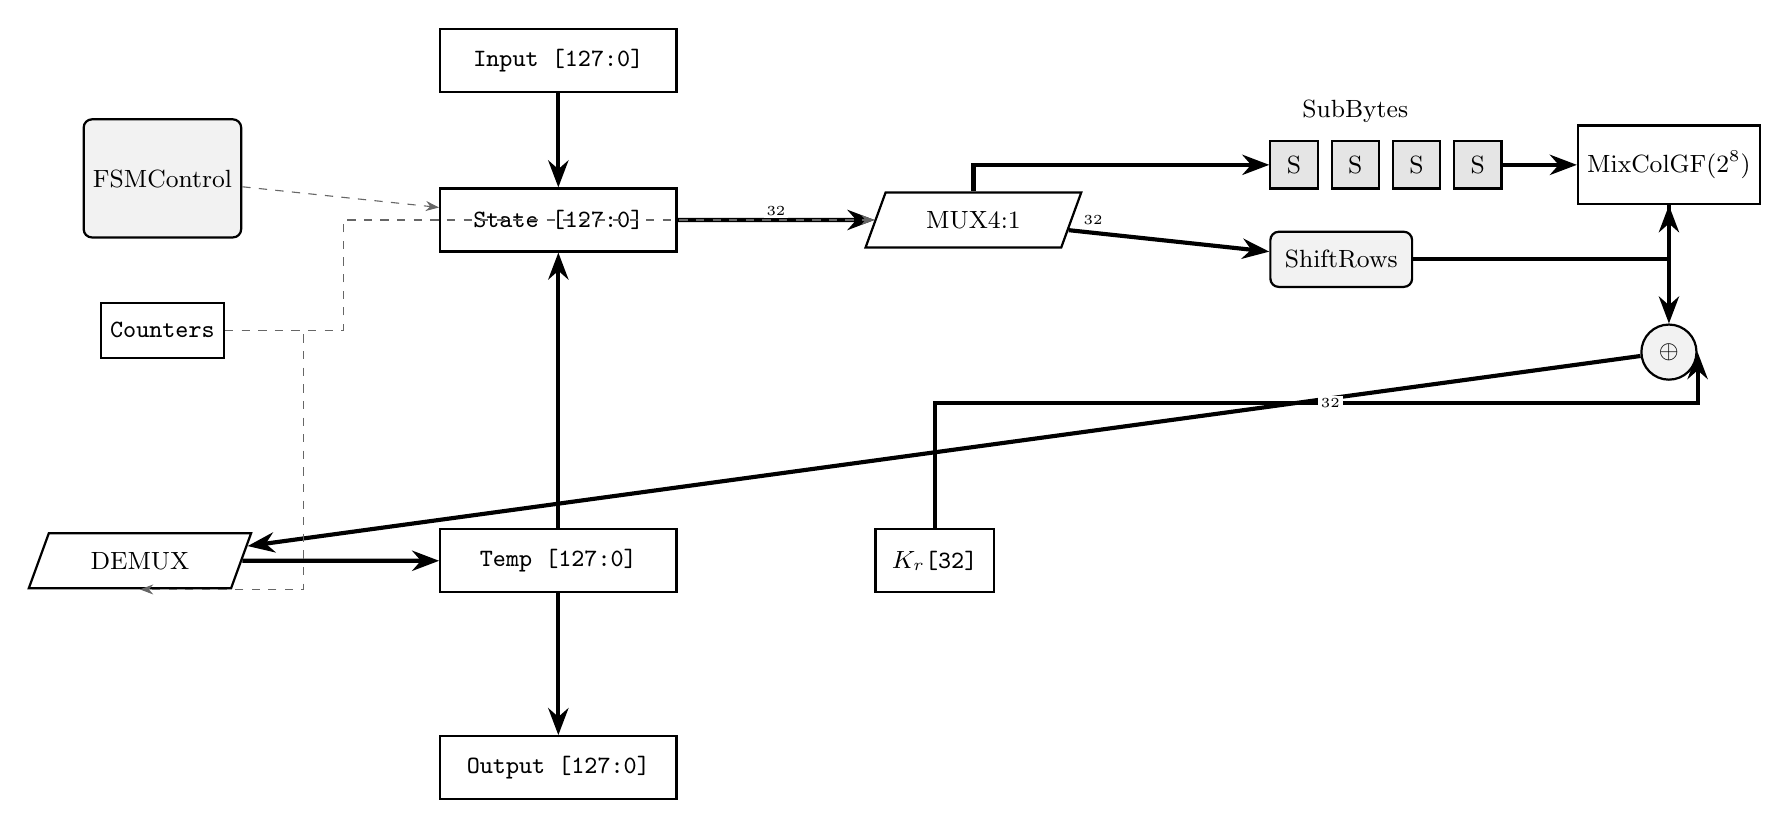
\begin{tikzpicture}[node distance=1.5cm and 2cm]

% Control FSM (left side)
\node[logic, minimum width=2cm, minimum height=1.5cm] (fsm) at (0,0) {FSM\\Control};
\node[register, minimum width=1.2cm, minimum height=0.7cm, below=0.8cm of fsm] (counters) {Counters};

% State registers (vertical column)
\node[register, minimum width=3cm, right=2.5cm of fsm, yshift=1.5cm] (input_reg) {Input [127:0]};
\node[register, minimum width=3cm, below=1.2cm of input_reg] (state_reg) {State [127:0]};
\node[register, minimum width=3cm, below=3.5cm of state_reg] (temp_reg) {Temp [127:0]};
\node[register, minimum width=3cm, below=1.8cm of temp_reg] (output_reg) {Output [127:0]};

% Column MUX
\node[mux, right=2.5cm of state_reg, minimum width=1cm] (col_mux) {MUX\\4:1};
\node[buswidth, right=0.1cm of col_mux] {32};

% SubBytes S-boxes
\node[sbox, right=2.5cm of col_mux, yshift=0.7cm] (sbox0) {S};
\node[sbox, right=0.15cm of sbox0] (sbox1) {S};
\node[sbox, right=0.15cm of sbox1] (sbox2) {S};
\node[sbox, right=0.15cm of sbox2] (sbox3) {S};
\node[font=\small, above=0.1cm of sbox1] {SubBytes};

% ShiftRows
\node[logic, right=2.5cm of col_mux, yshift=-0.5cm, minimum width=1.8cm] (shift) {ShiftRows};

% MixColumns
\node[alu, right=2.5cm of sbox1, minimum width=1.5cm, minimum height=1cm] (mixcol) {MixCol\\GF($2^8$)};

% XOR (AddRoundKey)
\node[logic, circle, minimum size=0.7cm, below=1.5cm of mixcol] (xor) {$\oplus$};

% DEMUX
\node[mux, left=2.5cm of temp_reg, shape border rotate=180, minimum width=1cm] (demux) {DEMUX};

% Round key input
\node[register, minimum width=1.5cm, right=2.5cm of temp_reg] (key_word) {$K_r$[32]};

% Data flow arrows
\draw[bus] (input_reg) -- (state_reg);
\draw[bus] (state_reg) -- node[buswidth, above] {32} (col_mux);
\draw[bus] (col_mux.north) |- (sbox0.west);
\draw[bus] (sbox3) -- (mixcol);
\draw[bus] (col_mux) -- (shift);
\draw[bus] (shift.east) -| (mixcol.south);
\draw[bus] (mixcol) -- (xor);
\draw[bus] (xor) -- (demux);
\draw[bus] (demux) -- (temp_reg);
\draw[bus] (temp_reg.north) -- (state_reg.south);
\draw[bus] (temp_reg) -- (output_reg);

% Key path
\draw[bus] (key_word) -- ++(0,2) -| node[buswidth, near start, right] {32} (xor.east);

% Control signals
\draw[controlwire] (fsm) -- (state_reg);
\draw[controlwire] (counters.east) -- ++(1.5,0) |- (col_mux.west);
\draw[controlwire] (counters.east) -- ++(1,0) |- (demux.south);

\end{tikzpicture}
\end{document}
